\documentclass[../main.tex]{subfiles}

\begin{document}
	Die letzte in dieser Studienarbeit betrachtete Hardwarearchitektur ist die Grafikkarte (GPU). Moderne GPUs werden nicht nur zur Berechnung der auf dem Monitor gezeigten Inhalte genutzt, sondern können aufgrund ihrer Architektur auch für komplexe mathematische bzw. numerische Berechnungen genutzt werden. Die Vorzüge der Grafikkarte als Hilfsmittel zur Implementierung eines CNN und allgemein für aufwändige Rechenoperationen soll Abschnitt \ref{sec:cuda_berechnung} dieses Kapitels erläutert werden. Außerdem soll die Programmierung der Rechenoperationen auf GPUs am Beispiel von NVIDIAs CUDA-Umgebung gezeigt werden. Die Abschnitte \ref{sec:cuda_titan} \nameref{sec:cuda_titan} und \ref{sec:cuda_umsetzung} \nameref{sec:cuda_umsetzung} zeigen dann die in dieser Arbeit genutzte Hardware sowie den verfolgten Implementierungsansatz für ein Convolutional Neural Network. Leider konnte die Implementierung eines funktionsfähigen und lernenden CNNs auf CUDA nicht in der vorgegebenen Zeit beendet werden. Das entstandene System ist nicht in der Lage, die Muster des MNIST-Datensatzes korrekt zu klassifizieren. Der Fehler muss dabei in der Implementierung liegen, da das verwendete Netz in anderen Implementierungen ihren Zweck erfüllt und gute Ergebnisse in der Klassifizierung erzielt.
\section{Grafikkarten zur Berechnung} \label{sec:cuda_berechnung}
Der ursprüngliche Zweck von Grafikkarten war die Shader-Berechnung und damit waren GPUs ein dediziertes Werkzeug zur Berechnung der auf dem Bildschirm dargestellten Inhalte. Da aufwändige grafische Darstellungen auch viele Berechnungen für die steigende Zahl an Pixel bedeuten, haben sich Grafikkarten zu hochparallelen Recheneinheiten entwickelt. Ihre Möglichkeiten sind dabei im Vergleich zu general-purpose CPUs eingeschränkt, jedoch sind sie auf komplexe Matrixoperationen im \emph{floating point} -Format ausgelegt. Dabei besitzen sie eine Vielzahl an Rechenkernen, womit es möglich wird, eine große Masse an mathematischen Operationen parallel zu bearbeiten. \par Dieser Abschnitt beschäftigt sich mit der Programmierung von mathematischen Anwendungen auf Grafikkarten, im speziellen mit der CUDA-Programmierung und weist im Punkt \ref{sec:cuda_cublas} auf eine hilfreiche, von NVIDIA bereitgestellte Bibliothek hin. \par 
\subsection{Stärken und Schwächen der Grafikkarte} \label{sec:cuda_staerken}
Wie bereits erwähnt, sind moderne Grafikkarten in der Lage komplexe mathematische Operationen äußerst effizient durchzuführen, da sie über eine hohe Zahl an Recheneinheiten verfügen. Aktuelle Hochleistungs-Grafikkarte besitzen mehrere Tausend Rechenwerke. Im Fall von NVIDIAs CUDA werden diese \emph{CUDA-Cores} genannt. Der offensichtliche Vorteil der Verwendung von Grafikkarten für aufwändige Berechnungen liegt in der gegebenen hohen Parallelität (vgl. \cite{NVIDIA_HOMEPAGE}). GPUs verfügen dabei aber nicht über den Instruktionsumfang gängiger CPUs. Generell kann festgestellt werden, das GPUs nicht für komplex verschachtelte Programmabläufe geeignet sind. Sie sind auf Rechenoperationen spezialisiert und eignen sich nur bedingt für andere Programmabläufe. Speziell besitzen Grafikkarten nur bedingte Möglichkeiten zur \emph{branch prediction} (Verzweigungsvorhersage). \par Außerdem benötigen GPUs immer eine CPU, die Rechenoperationen oder Programme auf der Grafikkarte startet und diese kontrolliert und koordiniert. Ein weiterer entscheidender Nachteil von modernen leistungsstarken Grafikkarten ist ihr hoher Preis. Im Vergleich zu hochwertigen CPUs sind Grafikkarten sehr teuer. Der Einsatz von GPUs für mathematische Berechnungen ist daher nur sinnvoll, wenn eine hohe Zahl an Rechenoperationen notwendig ist oder eine große Datenmenge im Sinne von Berechnungen verarbeitet werden muss. Das Problem muss sich dabei auch geeignet parallelisieren lassen, da sonst der Vorteil der Grafikkarte erlischt. \par Der nächste Abschnitt \ref{sec:cuda_unterschiede} soll die allgemeine Architektur einer modernen NVIDIA CUDA-fähigen Grafikkarte darstellen und damit den hier erwähnten Vorteil der Parallelität unterstreichen. \par 
\subsection{Architektur moderner Grafikkarten} \label{sec:cuda_unterschiede}
Prinzipiell sind die Architekturen der aktuellen NVIDIA Grafikkarten gleich aufgebaut. Eine Grafikkarte besteht dabei aus \emph{Streaming Multiprocessors (SM)}, den CUDA-Cores, einem dedizierten Graphikspeicher mit entsprechenden Caches und Speicher-Controllern. \par 
\begin{figure}[!htbp]
	\centering
	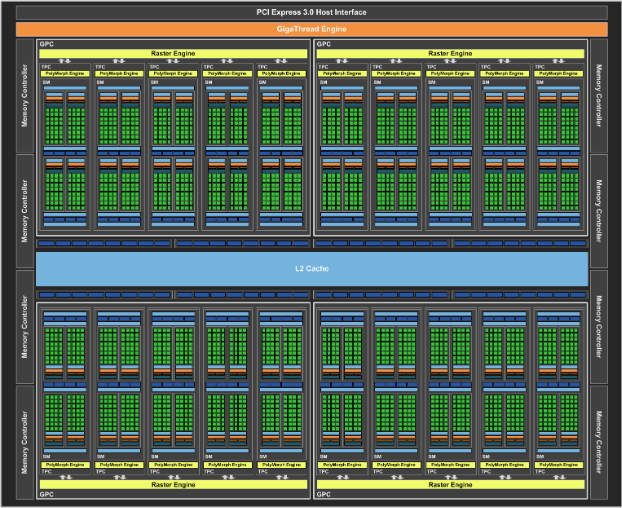
\includegraphics[width=0.8\linewidth]{../images/Riedle/architektur_pascal_komplett.png}
	\caption{Grafikkartenarchitektur am Beispiel der Pascal-Architektur von NVIDIA ( \cite{Pascal_white})} \label{pic:cuda_pascal_compl}
\end{figure}
Abbildung \ref{pic:cuda_pascal_compl} zeigt die erwähnten Komponenten in ihrem Zusammenspiel am Beispiel der Pascal-Architektur von NVIDIA. Diese findet beispielsweise in Grafikkarten vom Typ GTX 1080 Ti Anwendung. Von oben beginnend, ist in Abbildung \ref{pic:cuda_pascal_compl} die PCIe-Schnittstelle zum Host-System gezeigt. Das Host-System bildet die bestimmende CPU. Darunter folgt die GigaThread-Engine. Weiter ist die GPU in GPCs (Graphic Processing Clusters) unterteilt. Diese besitzen je eine Raster Engine und greifen auf den selben L2-Cache zu (vgl. \cite{Pascal_white}). Die GPCs sind weiter unterteilt in je zehn SMs.  Die Streaming Multiprocessors teilen die Arbeit auf in dieser Architektur 128 CUDA-Cores auf. Jede SM besitzt dabei eine separaten L1-Cache. \par 
\begin{figure}[!htbp]
	\centering
	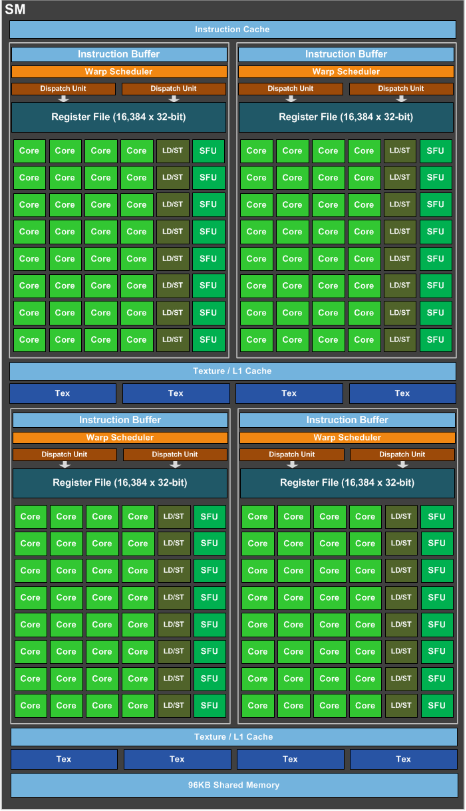
\includegraphics[width=0.8\linewidth]{../images/Riedle/architektur_pascal.png}
	\caption{Aufbau eines Streaming Multiprocessors in der Pascal-Architektur (\cite{Pascal_white})} \label{pic:cuda_sm}
\end{figure}
In Abbildung \ref{pic:cuda_sm} ist eine detaillierte Darstellung einer SM gegeben (vgl. \cite{Pascal_white}). Ein Streaming Multiprocessor besteht dabei aus vier Blöcken, auf die sich die 128 CUDA-Cores pro SM aufteilen. In der Abbildung sind zur besseren Übersicht weniger Cores aufgetragen. Jeder dieser Blöcke besitzt einen dedizierten \emph{Instruction Buffer}, einen \emph{Warp Scheduler} und ein sogenanntes \emph{Register File}. Darin sind 16384 32-Bit Register abgebildet. \par 
Ein Warp ist in CUDA eine Einheit von 32 Threads. Die CUDA-Struktur bildet alle erzeugten Threads in solche Warps ab und verteilt diese entsprechend innerhalb eines SM. Außerdem besitzt jede SM zwei L1-Caches und acht \emph{Texture Units}. Des weiteren besitzt jeder Streaming Multiprocessor einen dedizierten Shared-Memory-Bereich.\par 
Nachdem nun in diesem Abschnitt auf die grundlegende Architektur von NVIDIAs Grafikkarten am Beispiel der Pascal-Architektur eingegangen wurde, soll im Abschnitt \ref{sec:cuda_programmierung} auf einige Aspekte der CUDA-Bibliothek und damit der Programmierung von Anwendungen auf CUDA-fähigen Grafikkarten eingegangen werden. Die als Zielhardware für diesen Projektteil verwendete NVIDIA GTX Titan X Grafikkarte ist mit der sogenannten Maxwell Architektur ausgestattet. Diese wird in Abschnitt \ref{sec:cuda_titan} näher erläutert. \par 
\subsection{CUDA Programmierung} \label{sec:cuda_programmierung}
Die CUDA-Programmierung basiert auf der Programmierung von sogenannten \emph{Kernels}. Ein Kernel stellt dabei eine Routine dar, welche auf einer GPU ausgeführt werden kann. \par 
\begin{lstlisting}[language=C, caption=Minimaler Kernel, captionpos=b, label=listing:min_kernel]
	__global__ void minimal_kernel(float* a, float* b, float* c, 
									int size)
	{
		for(int i = 0; i < size; i++)
		{
			c[i] = a[i] + b[i];
		}		
	}
\end{lstlisting}
Listing \ref{listing:min_kernel} zeigt einen simplen CUDA-Kernel. Dieses Minimalbeispiel nimmt drei Zeiger auf \texttt{floats} und eine Ganzzahl als Parameter. Er addiert dabei einfach elementweise die Inhalte der Arrays \texttt{a} und \texttt{b} und speichert das Ergebnis im Array \texttt{c}. Im momentanen Zustand wird die \texttt{for} -Schleife seriell auf der GPU ausgeführt. Zur Parallelisierung später in diesem Abschnitt mehr. Wichtig ist hier der Specifier \texttt{\_\_global\_\_}. Er definiert einen CUDA-Kernel. Solche Kernels können nun vom Host aus auf der Grafikkarte gestartet werden (vgl. \cite{CUDA_GUIDE}). Der Host ist in jedem Fall die CPU und der darauf laufende Teil des Programmcodes. Mit dem Specifier \texttt{\_\_device\_\_} können Subroutinen auf der GPU deklariert werden. Solche Funktionen dürfen nur von Kernels auf der GPU aufgerufen werden. \\ Es ist zu beachten, dass die übergebenen Arrays \texttt{a}, \texttt{b} und \texttt{c} auf im Speicher der GPU liegen müssen. Die Grafikkarte hat keinen direkten Zugriff auf den RAM des Systems. Es muss also immer ein Transfer der Daten vom Host über die PCIe-Schnittstelle des Systems auf das Device (Grafikkarte) und zurück erfolgen. Dazu bietet die CUDA- Library spezielle Funktionen an. \par 
Bei der CUDA- Library handelt es sich um eine C/C++ -Bibliothek. Diese stellt verschiedene Funktionen zur Kommunikation und Kontrolle der GPU vom Host aus zur Verfügung. Wichtige Funktionen stellen dabei die Methoden \texttt{cudaMalloc(..)}, \texttt{cudaFree(..)} und \texttt{cudaMemcpy(..)} dar. Damit wird der Zugriff auf den Speicher der Grafikkarte vom Host aus geregelt. \par 
\begin{lstlisting}[language=C, caption=Aufruf des minimalen Kernels mit Speicherzugriff vom Host, captionpos=b, label=listing:min_kernel_host, breaklines]
	float *A_host, *B_host, *C_host;
	float *A_device, *B_device, *C_device;
	
	A_host = malloc(ARRAY_SIZE_D*sizeof(float));
	B_host = malloc(ARRAY_SIZE_D*sizeof(float));
	C_host = malloc(ARRAY_SIZE_D*sizeof(float));
	
	fillArrays(A_host, B_host, ARRAY_SIZE_D); /* Hilfsroutine, um den Arrays Werte zuzuweisen */
	
	cudaStatus_t cuda_state;
	
	cuda_state = cudaMalloc((void**) &A_device, ARRAY_SIZE_D*sizeof(float));
	cuda_state = cudaMalloc((void**) &B_device, ARRAY_SIZE_D*sizeof(float));
	cuda_state = cudaMalloc((void**) &C_device, ARRAY_SIZE_D*sizeof(float));
	
	cuda_state = cudaMemcpy((void*) A_device, (void*) A_host, ARRAY_SIZE_D*sizeof(float), cudaMemcpyHostToDevice);
	cuda_state = cudaMemcpy((void*) B_device, (void*) B_host, ARRAY_SIZE_D*sizeof(float), cudaMemcpyHostToDevice);
						
	minimal_kernel<<<1,1>>>(A_device, B_device, C_device);
	
	cuda_state = cudaMemcpy((void*) C_host, (void*) C_device, ARRAY_SIZE_D*sizeof(float), cudaMemcpyDeviceToHost);
	
	cuda_state = cudaFree((void*) A_device);
	cuda_state = cudaFree((void*) B_device);
	cuda_state = cudaFree((void*) C_device);
\end{lstlisting}
In Listing \ref{listing:min_kernel_host} ist ein Beispiel zur Nutzung des in Listing \ref{listing:min_kernel} beschriebenen Kernels zu sehen. Es werden zuerst host-seitig Pointer zu Speicheradressen auf dem Host und auf der Grafikkarte angelegt. Mit Hilfe der bekannten C Standardfunktion \texttt{malloc(..)} werden Arrays von Gleitkommazahlen auf dem Host reserviert. In einer zu definierenden Hilfsfunktion werden diese Speicherbereiche mit sinnvollen Werten beschrieben. Danach wird Speicher auf der GPU reserviert. Dazu wird die Funktion \texttt{cudaMalloc(..)} aus der CUDA-Library verwendet. Diese weist dem bereits angelegten Pointer auf dem Host eine Speicheradresse auf der Grafikkarte zu. Als Parameter fordert diese Funktion den besagten Zeiger im Format \texttt{void**} und die Größe des benötigten Speicherbereichs in Byte. Das \texttt{void**} -Format macht sowohl einen Cast als auch eine erneute Referenzierung des Pointers notwendig. \\ Der Rückgabewert aller hier genannten Funktionen der CUDA-Bibliothek ist vom Typ \texttt{cudaStatus\_t}. Dieser informiert über den Erfolg des Funktionsaufruf. Er ist besonders hilfreich zu Debug-Zwecken. Beispielsweise werden auch fehlerhafte Aufrufe im Sinne der Übergabe von Speicheradressen auf dem Host in diesem Rückgabewert vermerkt. \par Nachdem der Speicherplatz für die Arrays nun auch auf der GPU reserviert wurde, müssen nun die Werte der auf dem Host bereits belegten Arrays auf die Grafikkarte übertragen werden. Dazu steht die Funktion \texttt{cudaMemcpy(..)} zur Verfügung. Diese regelt den Zugriff auf den Speicherbereich der GPU über die PCIe-Schnittstelle. Die Methode benötigt vier Paramater. Sie fordert zwei Pointer als Ziel- und Quelladresse in genannter Reihenfolge, sowie die Anzahl der zu übertragenen Bytes. Bis zu diesem Zeitpunkt stimmt die Syntax mit der aus der C-Standardbibliothek bekannten \texttt{memcpy(..)} -Methode überein. Der vierte Paramater der CUDA-Methode legt nun die Übertragungsrichtung fest. Er bestimmt, ob vom Host zur Grafikkarte (\texttt{cudaMemcpyHostToDevice}), von der GPU zum Host (\texttt{cudaMemcpyDeviceToHost}) oder von Speicheradressen auf der Grafikkarte zu anderen dort befindlichen Speicherbereichen (\texttt{cudaMemcpyDeviceToDevice}). \par Anschließend folgt der Kernel-Aufruf. Hier taucht die spezielle CUDA-Syntax zum Kernel-Aufruf auf. In CUDA müssen Kernel beim Aufruf zwei zusätzliche Parameter in drei spitzen Klammern (\texttt{<<<1,1>>>}) übergeben werden. Diese bestimmen die Parallelisierung des Kernels, in dem Sie die Anzahl der vom Kernel verwendeten Threads festlegen. \\ Threads sind dabei in CUDA in Blöcken organisiert. Der zweite angegebene Paramter in den spitzen Klammern legt dabei die Anzahl der vom Kernel zu startenden Threads pro Block fest. Der erste Parameter bestimmt die Anzahl der zu verwendenden Blöcke. Diese Blöcke sind dabei in einem sogenannten Grid organisiert (vgl. \cite{CUDA_GUIDE}). \par 
\begin{figure}[!htbp]
	\centering
	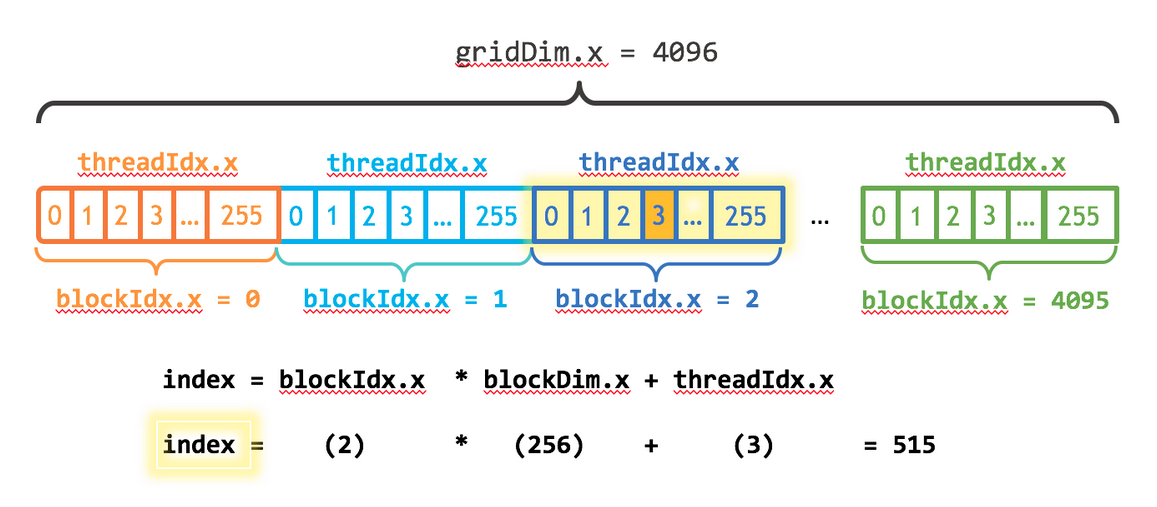
\includegraphics[width=\linewidth]{../images/Riedle/cudaThreadGridExample.png}
	\caption{Exemplarische Darstellung des Aufbaus eines Thread-Grids (\cite{CUDA_GUIDE})} \label{pic:cuda_threadExample}
\end{figure}
In Abbildung \ref{pic:cuda_threadExample} ist ein exemplarischer Aufbau eines solchen Thread-Grids gezeigt. Darin sind je 256 Threads pro Block und 4096 Blöcke im Grid abgebildet. Der zugehörige Aufruf gestaltet sich wie in Listing \ref{listing:cuda_kernel_threadExample} gezeigt. \par 
\begin{lstlisting}[language=C, caption=Aufruf des minimalen Kernels mit 4096 Blöcken à 256 Threads , captionpos=b, label=listing:cuda_kernel_threadExample, breaklines]
	minimal_kernel<<<4096,256>>>(A_device, B_device, C_device);
\end{lstlisting}
In dem dort dargestellten Beispiel würde mit der in Listing \ref{listing:min_kernel} gezeigten Implementierung des \texttt{minimal\_kernel(..)} jeder der erzeugten Threads die gleichen Berechnungen redundant ausführen. Bis zu diesem Punkt ist keine konkrete Parallelisierung vorgenommen worden. Um nun die Berechnungen unter den Threads zu verteilen kann eine Modifizierung des Kernels nach Listing \ref{listing:cuda_parallel_kernel} vorgenommen werden. 
\begin{lstlisting}[language=C, caption=Parallelisierte Variante des Kernels , captionpos=b, label=listing:cuda_parallel_kernel, breaklines]
	__global__ void minimal_kernel(float *a, float *b, float *c, int size)
	{
		int index = blockIdx.x * blockDim.x + threadIdx.x;
		int stride = blockDim.x * gridDim.x;
		
		for(int i = index; i < size; i+=stride)
		{
			c[i] = a[i] + b[i];
		}
	}
\end{lstlisting}
Die hier verwendete Methode der Parallelisierung wird \emph{grid-stride-loop} genannt (vgl. \cite{CUDA_GRID_STRIDE}). Damit wird die Berechnung flexibel auf die angegebenen Thread-Parameter angepasst. Jeder Thread berechnet hierbei seinen Index nach der Formel \texttt{index = blockIdx.x * blockDim.x + threadIdx.x;}. Die CUDA-Library stellt dazu die Strukturen \texttt{blockIdx}, \texttt{blockDim} und \texttt{threadIdx} zur Verfügung. Darin sind die jeweiligen Thread-Parameter des Aufrufs gespeichert. In der \texttt{for} -Schleife wird die Laufvariable dann mit dem berechneten Index initialisiert. Die Sprungweite der Laufvariable wird durch die Variable \texttt{stride} bestimmt. Diese stellt die Anzahl aller verwendeten Threads in allen Blöcken dar. Sie ist damit das Produkt aus Anzahl der Blöcke und Anzahl der Threads pro Block. Durch die Nutzung der \emph{grid-stride-loop} wird nun jeder Wert des Ausgangsarrays \texttt{c} nur in einem Thread berechnet. Jeder Thread schreitet in der Schleife das Array mit der Anzahl aller Threads als Sprungweite ab, jeweils versetzt um seine Position im Grid. \par Damit sind nun die Grundlagen der CUDA-Programmierung und der damit möglichen Parallelisierung behandelt. In Abschnitt \ref{sec:cuda_umsetzung} wird nachfolgend beschrieben, wie diese Mechanismen auf das vorliegende Problem der Parallelisierung eines CNNs angewendet wurden. \par 
\subsection{cuBLAS und cuRand} \label{sec:cuda_cublas}
Die CUDA-Umgebung bietet neben der zwingend notwendigen CUDA-Runtime-Library weitere Bibliotheken zur Unterstützung an. Beispielsweise werden Bibliotheken für numerische Berechnungsmethoden oder auch die Implementierung von Deep Neural Networks angeboten. In diesem Projekt wurden zwei dieser Libraries verwendet, die cuBLAS-Bibliothek und die cuRand-Library in der Kernel-Version. \par Die cuBLAS-Bibliothek stellt eine auf NVIDIA GPUs spezialisierte Implementierung der BLAS-Funktionen zur Verfügung. Daraus wurde das Skalarprodukt für Vektoren benutzt. Die cuRand-Library bietet verschiedene Methoden zur Erzeugung von Zufallszahlen mit GPU-Unterstützung an. Sie existiert sowohl als Host-Version, als auch als für Kernel geeignete Version. Sie wurde verwendet, um in einem Kernel die Initialwerte des Gewichte und Biases des Neuronalen Netzes zufällig zu bestimmen. \par 
\section{Verwendete Hardware: GTX Titan X} \label{sec:cuda_titan}
Die Implementierung und Parallelisierung des Convolutional Neural Networks in dieser Arbeit ist auf die Verwendung auf Systemen mit einer NVIDIA Geforce GTX Titan X ausgelegt. Diese stand auf einem Server der Dualen Hochschule Baden-Württemberg Stuttgart zur Verfügung. Sie ist mit 3072 CUDA-Cores ausgestattet. Dies erlaubt einen äußert hohen Grad der Parallelisierung. Außerdem verfügt die GTX Titan X über 12 GB dedizierten VRAM. Dadurch ist es Möglich, große Datenmenge ohne häufige externe Speicherzugriffe zu verarbeiten. \par Die GTX Titan X ist dabei wie bereits in Abschnitt \ref{sec:cuda_unterschiede} \nameref{sec:cuda_unterschiede} erwähnt nach der Maxwell -Architektur aufgebaut. Auch diese Architektur stützt sich auf \emph{Streaming Multiprocessors}, welche hier SMM genannt werden. Die GTX Titan X verfügt dabei über 24 solcher SMMs mit je 128 CUDA-Cores. Auch hier teilen sich die SMMs die gleichen Komponenten, wie bereits in Abschnitt \ref{sec:cuda_unterschiede} anhand der Pascal-Architektur erläutert wurde. Der wesentliche Unterschied liegt im Aufbau er SMM. \par 
\begin{figure}[!htbp]
	\centering
	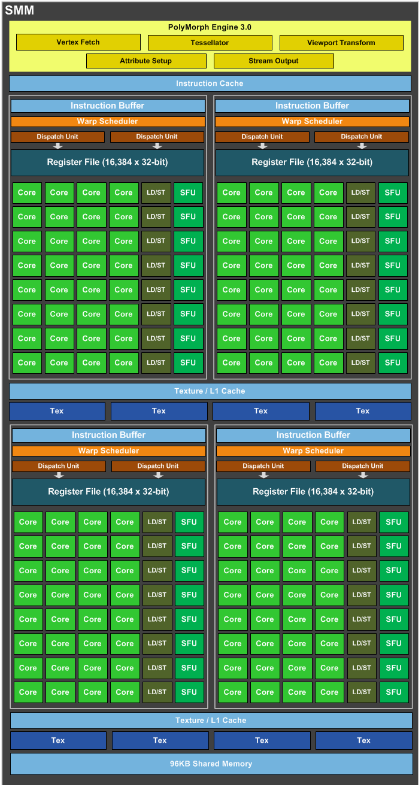
\includegraphics[width=0.6\linewidth]{../images/Riedle/Maxwell_SMM_Single.png}
	\caption{Aufbau einer Maxwell SMM \cite{CUDA_MAXWELL_white}} \label{pic:cuda_maxwell_smm_single}
\end{figure}
Diese Aufbau ist in Abbildung \ref{pic:cuda_maxwell_smm_single} dargestellt. Jede SMM verfügt über vier Warp-Scheduler. Damit ist es möglich, vier Warps pro SMM konkurrierend zu betreiben. Jeder Warp-Scheduler kontrolliert dabei 32 CUDA-Cores. Die L1-Caches unterscheiden sich nicht von der, der Pascal-Architektur. Auch die Register-Files sind unverändert, wodurch jedem Warp-Scheduler bzw. den darin organisierten CUDA-Cores 16384 32-Bit Register zur Verfügung stehen. Eine weitere Neuerung ist die Verlegung der \emph{PolyMorph Engine 3.0} direkt in die SMM. In der Pascal -Architektur befand sich diese noch außerhalb der SM. \par 
Es wurden nun alle relevanten Grundlagen der Programmierung auf CUDA sowie der Aufbau und die Struktur der verwendeten Hardware erläutert. Der nächste Abschnitt widmet sich der Implementierung des in dieser Arbeit vorgestellten Convolutional Neural Network unter Zuhilfenahme einer NVIDIA Geforce GTX Titan X Grafikkarte. Es werden der gewählte Ansatz zur Parallelisierung der Berechnungen, ein Ansatz zur Umsetzung der Faltung und die daraus resultierenden Änderungen in den weiteren Schichten des Netzes dargestellt. \par 

\section{Umsetzung und Parallelisierung} \label{sec:cuda_umsetzung} 
Die Stärke der Grafikkarte liegt in der effizienten Berechnung von mathematischen Operationen auf Matrizen. Folgend dieser Prämisse wurde bei der Umsetzung ein Ansatz gesucht, welcher die Berechnung der einzelnen Schichten durch geschickte Matrixoperationen abbilden kann. Es wurden im Vorfeld der Implementierung verschiedene Ansätze betrachtet. Darunter der \emph{Winograd Small Convolution} -Algorithmus erweitert auf große Matrizen (vgl. \cite{WINOGRADSMALLCONV}) und eine auf der Fast-Fourier-Transformation basierende Methode (vgl. \cite{NVIDIA_WHITE_FFTCONV}). Die Wahl fiel dabei aufgrund von Recherchen von bereits bestehenden Vergleichen (vgl. \cite{UNROLLING_CONV}) auf die Methode der \emph{Unrolling based Convolution}. Damit ist es möglich, die Faltungsoperation eines Convolutional Neural Networks als einfache Matrix-Matrix-Multiplikation darzustellen. Diese Methode wird in \fref{sec:cuda_unrolling_conv} näher erläutert. \\ Die Unrolling-based Convolution hat nicht nur Einfluss auf die Convolutional Layer des Netzes, sonder auch auf die Pooling Layer und den Input Layer. Das in dieser Arbeit verwendete bereits in anderen Anwendungen erprobte Netz besteht aus einem Input Layer, zwei Convolutional Layern mit Faltungskernen der Größe $5\times 5$, zwei Pooling Layern mit $2\times 2$-Bereichen, welche die Größe des Layers jeweils halbieren, einer Fully Connected Schicht mit 1024 Nodes und einer finalen Fully Connected Schicht mit 10 Nodes. In der ersten Convolutional Schicht werden 32 Feature Maps erzeugt. In der zweiten werden 64 Feature Maps erzeugt. Eine Darstellung des verwendeten CNNs ist in \fref{fig:matrixkonfiguration} abgebildet. Darin sind bereits die bei der Unrolling-based Convolution -Methode entstehenden Matrizen schematisch dargestellt. Die Abbildung zeigt in der unteren Hälfte die verwendeten Node-Matrizen, die in den jeweiligen Layern notwendig sind. Die obere Hälfte der Graphik enthält die Gewichtsmatrizen, welche zwischen den entsprechenden Layern angeordnet sind. Bei Leserichtung von links nach rechts sind hier Matrix-Matrix-Multiplikationen der Layer mit den jeweiligen Gewichtsmatrizen zu interpretieren. \fref{sec:cuda_unrolling_conv} soll nun die gewählte Methode der Unrolling-based Convolution erläutern und damit Klarheit in die Darstellung der \fref{fig:matrixkonfiguration} bringen. \par 
\begin{figure}[!htbp]
	\centering
\begin{tikzpicture}[scale=0.7]
	\draw (0,1) rectangle (2,5); %input
	\draw (3,1) rectangle (4,5); %conv1
	\draw (2,6) rectangle (3,6.5); %weight 1
	\draw (5,2.5) rectangle (8,3.5); %maxpooling1
	\draw (8,6) rectangle (9.2, 8); %weight2
	\draw (9,1) rectangle (10,2); %conv2
	\draw (11, 2.5) rectangle (13, 2.7); %maxpooling 2
	\draw (13, 6) rectangle (15, 8); %weight3 
	\draw (16, 2.5) rectangle (18, 2.7); %fullyconnected1
	\draw (19, 2.5) rectangle (19.4, 2.7); %fullyconnected2
	\draw (18, 6) rectangle (18.3, 8); %weight4
	
	\node at (0,7) (weights) {Weights};
	\node at (0,0) (input) {Input};
	\node at (3,0) (conv1) {Conv1};
	\node at (6,0) (max1) {MaxPooling1};
	\node at (9,0) (conv2) {Conv2};
	\node at (12,0) (max2) {MaxPooling2};
	\node at (16,0) (ful1) {Fully1};
	\node at (19,0) (final) {Final Layer};
\end{tikzpicture}
\caption{Darstellung der genutzten Matrizen} \label{fig:matrixkonfiguration}
\end{figure}

\subsection{Unrolling-based Convolution} \label{sec:cuda_unrolling_conv}
Unrolling-based Convolution für Convolutional Neural Networks wurde 2006 von Mitarbeitern der Firma Microsoft vorgestellt. Dabei handelt es sich um eine Methode um die Faltungsoperation in Convolutional Neural Networks in eine einfach zu realisierende Matrix-Matrix-Multiplikation zu überführen (vgl. \cite{UNROLLING_CONV}). Dieser Ansatz verfolgt grundlegend die Idee, die Faltungsoperation zu entfalten bzw. auszurollen. Im ersten Schritt muss der Input des betreffenden Layers umsortiert und einige Werte vervielfacht werden.  \fref{fig:cuda_unrolling_1} zeigt die Operation am Beispiel von drei $3\times 3$ -Input-Matrizen, sechs $2\times 2$ -Faltungskernen und zwei Output -Features. \par 
\begin{figure}[!htbp]
	\centering
	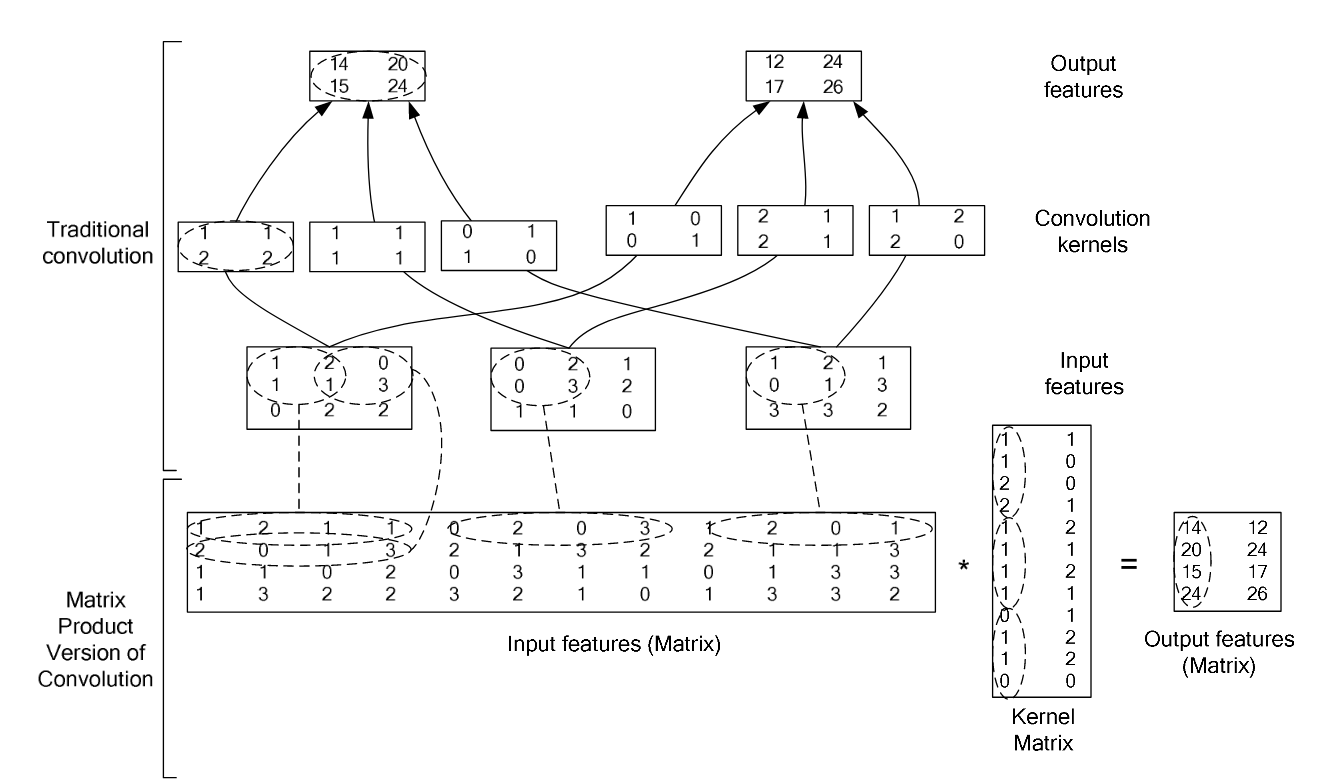
\includegraphics[width=0.8\linewidth]{../images/Riedle/Unrolling_1.png} \caption{Exemplarische Darstellung der Unrolling-based Convolution (vgl. \cite{UNROLLING_CONV})} \label{fig:cuda_unrolling_1}
\end{figure}
Das hier gezeigte Schaubild ist in zwei Bereiche unterteilt. Im oberen Teil ist die traditionelle Faltungsoperation abgebildet. Man sieht hier drei Input-Features der Größe $3\times 3$. Darüber sind sechs Gewichtsmatrizen der Faltungskerne mit den Ausmaßen $2\times 2$ gezeigt. Die Faltungsoperation führt dann zu zwei Output-Features der Größe $2\times2$. \\ Im unteren Teil der Graphik ist die zugehörige Unrolling-based Convolution abgebildet. Die drei Input-Features werden in eine Matrix umsortiert. Hierbei ist zu beachten, dass einige Werte der ursprünglichen Matrizen mehrfach auftreten. In dieser Abbildung ist die Zuordnung der den Faltungskernen entsprechenden Bereichen der ursprünglichen Matrizen in die neue ausgerollte Matrix anschaulich dargestellt. Auch die Faltungskerne selbst müssen in eine neue größere Matrix umsortiert werden. Dabei werden deren Gewichte pro Output-Feature in eine Spalte einer entstehenden Kernel-Matrix einsortiert. Auch dieser Schritt ist in \fref{fig:cuda_unrolling_1} überischtlich dargestellt. Wird nun die entstandene Input-Matrix mit der entstandenen Kernel-Matrix multipliziert, befinden sich in den Spalten der daraus entstehenden Output-Matrix die Werte der Output-Features. Die Output-Matrix kann nun in einem nächsten Schritt für eine weitere Convolutional Schicht erneut nach dem nun bekannten Schema umsortiert werden. Damit ist durch diesen Ansatz jede Schicht durch eine einfache Matrix-Matrix-Multiplikation darstellbar. Die Umsortierung der Eingangswerte in den jeweiligen Schichten ist dabei nach \cite{UNROLLING_CONV} signifikant weniger aufwändig, als die klassische Faltungsoperation. \par 
\begin{figure}[!htbp]
	\centering
	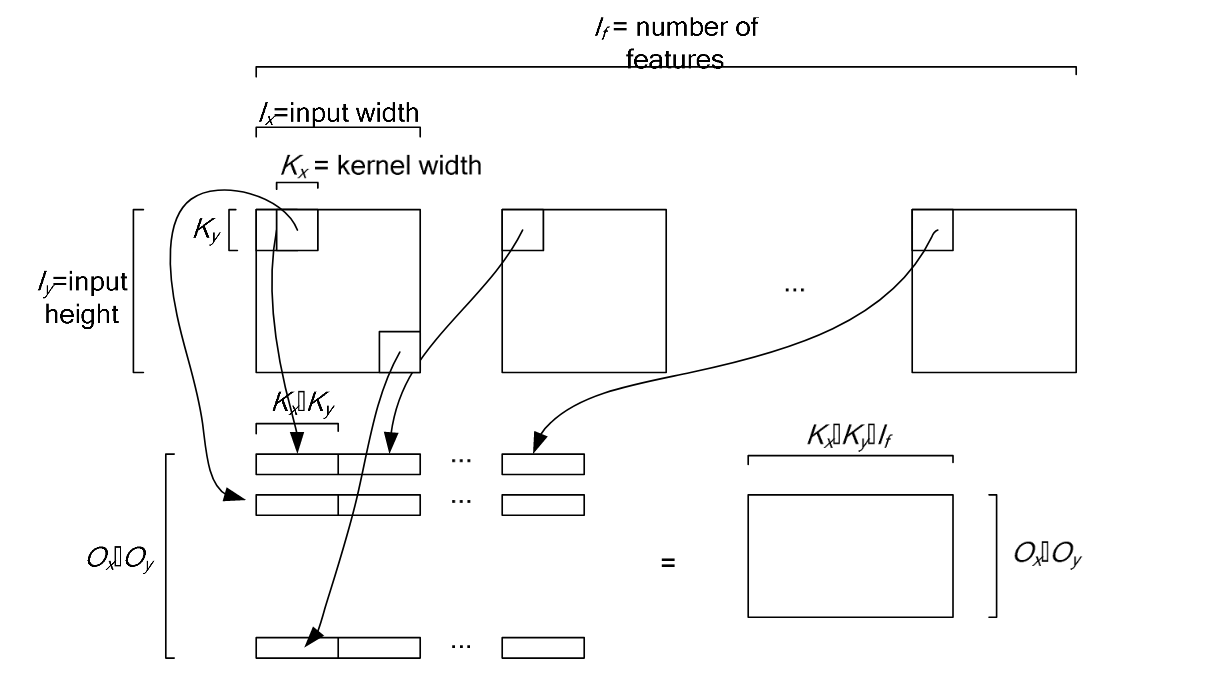
\includegraphics[width=0.8\linewidth]{../images/Riedle/Unrolling_2.png}
	\caption{Darstellung des Vorgangs der Umsortierung bei Unrolling-based Convolution (vgl. \cite{UNROLLING_CONV})} \label{fig:cuda_unrolling_2}
\end{figure}
Um die Größen der durch Unrolling-based Convolution entstehenden Matrizen zu bestimmen, kann das in \fref{fig:cuda_unrolling_2} gezeigte Schaubild zur anschaulichen Herleitung entsprechender Formeln dienen. Es zeigt den Vorgang der Umsortierung des Inputs eines Convolutional Layers. Dieser Input besteht aus $I_f$ Feature Maps, deren Matrixrepräsentationen jeweils $I_y$ Zeilen und $I_x$ Spalten aufweisen. Außerdem sind in den Input-Feature-Maps die Faltungskerne an verschiedenen Positionen aufgetragen. Diese Faltungskerne besitzen die Abmessungen $K_y \times K_x$. Vollzieht man nun die Operation der Umsortierung erhält man die Darstellung der unteren Hälfte der Abbildung. Die den Faltungskernen zugeordneten Werte werden pro Feature-Map jeweils in $K_x \cdot K_y$ Spalten der ausgerollten Matrix angeordnet. Es entsteht also eine Matrix mit $K_x\cdot K_y\cdot I_f$ Spalten. Die Anzahl der Zeilen dieser Matrix wird durch die Größe eines regulären Output-Features bestimmt. Diese bestimmt sich mit Schrittweite $1$ durch \fref{eq:cuda_output_feature_dim}.
\begin{align} \label{eq:cuda_output_feature_dim}
\begin{split}
	O_x = I_x -K_x + 1 \\
	O_y = I_y - K_y +1
\end{split}
\end{align}
Die umsortierte Matrix hat damit $O_x\cdot O_y$ Zeilen. Es ist also eine $(K_x\cdot K_y\cdot I_f) \times (O_x\cdot O_y)$ -Matrix entstanden. \par 
Nun müssen auch die Gewichte entsprechend in einer angepassten Matrix angeordnet werden. Dabei müssen in einer Spalte dieser Matrix die den Faltungskernen in den jeweiligen Input-Features zugeordneten Gewichte verortet sein. Jede Spalte ist dabei einem Output-Feature zugeordnet. \par 
\begin{figure}[!htbp]
	\centering
	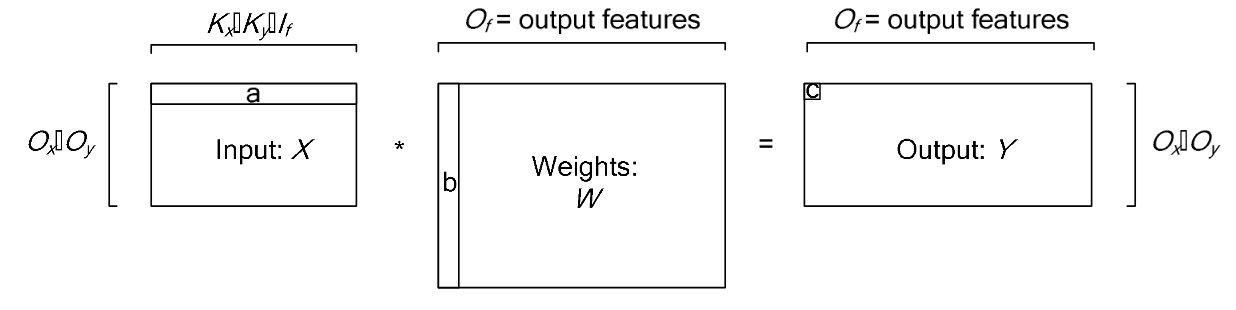
\includegraphics[width=\linewidth]{../images/Riedle/Unrolling_3.png}
	\caption{Veranschaulichung der sich ergebenden Matrixgrößen bei Unrolling-based Convolution (vgl. \cite{UNROLLING_CONV})} \label{fig:cuda_unrolling_3}
\end{figure}
\fref{fig:cuda_unrolling_3} zeigt den Vorgang der resultierenden Matrix-Matrix-Multiplikation. Darin sind zusätzlich die Dimensionen der jeweiligen Matrizen aufgetragen. Das Ergebnis der Multiplikation liefert eine Output-Matrix mit $O_x \cdot O_y$ Zeilen und $O_f$ Spalten. $O_f$ bezeichnet dabei die Anzahl der Output-Features. Darin sind wie bereits erwähnt, die jeweiligen entstehenden Feature-Maps durch die Spalten der Matrix repräsentiert. Das Skalarprodukt einer Input-Zeile $a$ mit einer Spalte $b$ der Gewichtsmatrix ergibt dabei ein Output-Node $c$, repräsentiert durch einen Wert in der Output-Matrix. \par 
Nachdem nun die Methode der Unrolling-based Convolution betrachtet wurde, sollen in den nächsten Abschnitten die Auswirkungen dieses Ansatzes auf die verschiedenen Layer eines Convolutional Neural Networks am Beispiel des in dieser Arbeit betrachteten Netzes dargestellt werden. \par 

\subsection{Input-Layer} \label{sec:cuda_input}
Entgegen den anderen in dieser Arbeit gezeigten Implementierungen ist mit dem gewählten Ansatz der Unrolling-based Convolution ein dedizierter Input-Layer notwendig. Dieser Layer stellt in der vorliegenden Implementierung die im Sinne der  Unrolling-based Convolution ausgerollte Matrix des Eingangsbildes dar. \par 
Dabei wird das $28\times 28$ Pixel große Input-Muster in dem hier betrachteten Netz derart umsortiert, dass eine $576\times 25$ -Matrix entsteht. Die Matrixdimensionen ergeben sich aus der Definition des nachfolgenden Convolutional Layers. Dieser besteht aus $5\times 5$ -Faltungskernen, was mit einer Schrittweite von $1$ zu einem $24\times24 = 576$ -Pixel großen Output führt. Dies findet natürlich 32 mal für jede in diesem Layer auftretende Feature Map statt. Die Anzahl der Zeilen im Input-Layer ergibt sich also durch die Größe einer Feature Map des folgenden Convolutional Layers. Die Schwierigkeit in diesem Layer lag in einem geeignet Algorithmus zur Zuordnung der Ausgangswerte in die neue ausgerollte Matrix. Listing \ref{listing:cuda_input} zeigt den in der Implementierung genutzten Algorithmus. \par \clearpage 
\begin{lstlisting}[language=C, caption=Umsortierung im Input-Layer , captionpos=b, label=listing:cuda_input, breaklines]

int size =  576; /*24x24*/

for(int n = index; n < size; n+=stride)
{
	int i = n/24; /*rows in original row-major picture*/
	int j = n%24; /*columns in original picture*/
	
	for(int k = 0; k < 5; k++) /*convolutional kernel rows in original picture*/
	{
		for(int l = 0; l < 5; l++) /*convolutional kernel columns in original picture*/
		{
			arrayPtr[(k*5+l)*576+i*24+j] = picturePtr[(i+k)*24+j+l];
		}
	}
}
\end{lstlisting}
Darin wird jeder Wert des Ausgabebildes in der Convolutional Schicht der klassischen Variante der Faltung in der äußersten Schleife abgeschritten. Anschließend die Position in diesem Originalbild in Form von Zeilen $i$ und Spalten $j$ bestimmt. Die beiden inneren Schleifen schreiten nun eine Zeile der neuen umsortierten Matrix ab, wobei diese befüllt mit den entsprechenden Werten des Eingabebildes befüllt. Auch hier ist eine \emph{Grid-Stride-Loop} umgesetzt. \par 

\subsection{Convolutional Layer} \label{sec:cuda_conv}
In den Convolutional Layern des CNN mit Unrolling-based Convolution entstehen wie bereits in \fref{sec:cuda_unrolling_conv} detailliert beschrieben Matrizen mit $x$ Zeilen und $y$ Spalten, wobei $x$ durch die Größe einer Feature Map und $y$ durch die Anzahl der Feature Maps bestimmt wird. Damit ist die für die erste Convolutional Schicht des betrachteten Convolutional Neural Network Node-Matrix von der Größe $576 \times 32$. Der zweite Convolutional Layer benötigt eine $64 \times 64$ Node-Matrix. Hier wird eine durch den vorhergehenden ersten MaxPooling Layer entstandene $12\times 12$ -Matrix mit einem Faltungskern der Dimension $5\times 5$ gefaltet. Diese Faltung wird auf 64 Feature Maps angewendet. \par In dieser Implementierung wurden die Gewichtsmatrizen den jeweils durch Multiplikation entstehenden Layern zugeordnet. Das bedeutet, die erste auftretende Gewichtsmatrix ist die, des ersten Convolutional Layers. Diese hat die Abmessungen $25\times 32$. Hier sind die Gewichtswerte der Faltungskerne für jede Feature Map in den Spalten der Matrix repräsentiert. Die Gewichtsmatrix des zweiten Convolutional Layers ist von der Größe $800 \times 64$, wobei die Anzahl der Spalten erneut durch die Zahl der Feature Maps des Convolutional Layers gegeben ist. Die Anzahl der Zeilen bestimmt sich nach \begin{align} \label{eq:cuda_spalten_pooling}
 K_x \cdot K_y \cdot I_f = 5\cdot5\cdot32 \end{align} und wird somit durch den vorhergehenden MaxPooling Layer bestimmt. Die in den Convolutional Layern durchgeführten Operationen beschränken sich dank der Methode der Unrolling-based Convolution auf einfache Matrix-Matrix-Multiplikationen. Der für diese Schicht vorgesehene CUDA-Kernel implementiert damit nur diese Matrix-Matrix -Multiplikation. Die notwendigen Umsortierungen werden bereits in den vorhergehenden Layern durchgeführt. Natürlich müssen hier auch die entsprechenden Biases addiert und die Aktivierungsfunktion angewendet werden. \par 

\subsection{MaxPooling-Layer} \label{sec:cuda_pooling}
In den MaxPooling Layern des Convolutional Neural Network wird die Größe der vorhergehenden Convolutional Schichten durch sogenanntes \emph{Subsampling} halbiert. Die Layer ermitteln jeweils das Maximum eines $2\times2$ -Bereichs. Dieser Wert wird weiter verwendet, der Rest wird verworfen. Damit ergeben sich im ersten MaxPooling Layer des hier gezeigten Neuronalen Netzes 32 Feature Maps mit einer Größe von je $12\times12$ Bildpunkten. In der zweiten MaxPooling Schicht befinden sich analog 64 Feature Maps mit einer Abmessung von $4\times4$. \par In den MaxPooling Schichten des hier implementierten Netzes findet zusätzlich zum Subsampling, falls nötig, auch die Umsortierung für die nachfolgende Schicht statt. Dies ist der Fall, wenn auf die MaxPooling Schicht eine weitere Convolutional Schicht folgt. In dem hier gezeigten Beispiel betrifft das nur den ersten MaxPooling Layer. Die Node-Matrix dieses Layers hat damit die Ausmaße $64\times800$. Die Anzahl der Zeilen wird erneut durch die Größe der Feature Maps des nachfolgenden Convolutional Layers bestimmt. Die Anzahl der Spalten berechnet sich wie bereits gezeigt nach \fref{eq:cuda_spalten_pooling}. \par Auch hierbei war die größte Schwierigkeit die Umsortierung der Matrix. Bei der Implementierung des MaxPooling Layers wird zuerst eine Hilfsmatrix erzeugt, welche die durch das Subsampling entstehende Matrix ohne Umsortierung darstellt. Diese enthält die entsprechenden Werte aller Feature Maps. Nach der Durchführung des Subsampling werden die Werte der Hilfsmatrix entsprechend in die eigentliche MaxPooling-Matrix einsortiert, sodass in der nachfolgenden Convolutional Schicht wieder nurmehr eine Matrix- Matrix -Multiplikation durchgeführt werden muss, um den Output dieser Schicht zu bestimmen. Für den Fall eines nachfolgenden Fully Connected Layers muss keine zusätzliche Umsortierung vorgenommen werden. Da hier alle nach dem Subsampling verbleibenden Werte in Form eines Vektors auf die Nodes der Fully Connected Schicht abgebildet werden, kann der Output des Subsamplings ohne Modifikation verwendet werden. Die Werte liegen bereits derart im Speicher, dass sie als Vektor aufgefasst und verwendet werden können. \par 

\subsection{Fully Connected Layer} \label{sec:cuda_fully}
In dem in dieser Arbeit verwendeten Netz befinden sich am Ende des Neuronalen Netzes zwei Fully Connected Layer. Der erste hat eine Größe von $1024$ Nodes. Der zweite und finale Layer besteht aus $10$ Outputnodes, welche die Klassifizierung der Inputs darstellen. Die gewählte Methode der Unrolling-based Convolution hat keinen Einfluss auf das Verhalten bzw. die Implementierung dieser Layer. In den Fully Connected Schichten werden die Input-Vektoren mit den Gewichtsmatrizen multipliziert, wodurch erneut ein Ausgangsvektor entsteht. Hierauf müssen offensichtlich noch die Biases addiert und die Aktivierungsfunktion angewendet werden. \par Die Gewichtsmatrix, welche dem ersten Fully Connected Layer zugeordnet ist, hat dementsprechend eine Größe von $
1024\times1024$, um die $1024$ Werte des vorhergehenden MaxPooling Layers auf die $1024$ Werte des Vektors der Fully Connected Schicht abzubilden. Dem Final Layer ist somit eine $1024\times10$ -Gewichtsmatrix zugeordnet. \par 
Auch die CUDA-Kernel, welche den Fully Connected Layern zugeordnet sind, beschränken sich auf Matrix -Matrix -Multiplikationen und das addieren der Biases sowie die Anwendung der Aktivierungsfunktion. \par 
\subsection{Parallelisierung} \label{sec:cuda_parallelisierung}
Durch die hohe Zahl an Rechenwerken, die der verwendeten Grafikkarte zur Verfügung stehen, ist ein hoher Grad der Parallelisierung möglich. Um die Leistungsfähigkeit der NVIDIA GTX Titan X möglichst gut ausnutzen zu können, muss das Ziel aller Überlegungen zur Parallelisierung sein, die nötigen Rechenoperation bestmöglich zu verteilen und eine große Zahl an Threads zu erzeugen, welche dann auf die CUDA-Cores verteilt werden können. \par 
Grundsätzlich sind mehrere Ansätze zur Parallelisierung eines Convolutional Neural Networks denkbar. Eine Möglichkeit stellt eine Muster-Parallelität dar. Dabei werden die notwendigen Berechnungen für mehrere MNIST-Bilder gleichzeitig auf der Grafikkarte durchgeführt. Hier ist es beispielsweise möglich, ein ganzes Batch parallel zu berechnen. Denkt man aber daran, dass der GTX Titan X 3072 CUDA-Cores zur Verfügung stehen, wird schnell klar, dass diese Methode nicht zielführend ist. Um die Grafikkarte entsprechend auszulasten, wäre eine große Batch-Size nötig, was den Lernprozess negativ beeinflussen würde. \par 
Ein anderer Ansatz wird durch den Modell-Parallelismus spezifiziert. Hierbei wird versucht die Rechenschritte innerhalb des Modells, also des Neuronalen Netzes, zu parallelisieren. Auch dabei sind mehrere Varianten denkbar. Beispielsweise könnten die Berechnungen in den einzelnen Schichten für jede Node parallel durchgeführt werden. Diese Methode würde offensichtlich einen hohen Grad der Parallelisierung erlauben. Implementiert man die Faltungsoperation im klassischen Sinn, ist diese Möglichkeit sicher in Betracht zu ziehen. Eine weitere denkbare Parallelisierungsart ist die Parallelisierung über Spalten der jeweils erzeugten Ausgangsmatrizen. Aufgrund der hier gewählten Implementierungsweise der Unrolling-based Convolution wurde in dieser Arbeit eben diese Art der Parallelisierung gewählt. Jedem Thread wird dabei die Aufgabe zugeordnet, für jeweils eine Spalte der Gewichtsmatrix das Skalarprodukt mit allen Zeilen der Input-Matrix durchzuführen. Auch die Addition der Biases und die Anwendung der Aktivierungsfunktion ist diesem Task zugeordnet. \par Die Parallelisierung wurde dabei mit Fokus auf die Convolutional Layer umgesetzt. Es werden in jedem Layer jeweils 64 Threads gestartet. Dies entspricht der Anzahl der Spalten bzw. der Feature Maps des zweiten Convolutional Layer. Auch die Berechnungen im Input Layer, den MaxPooling Layern und den Fully Connected Layern wird auf diese 64 Threads verteilt, um eine deterministische Anzahl an Threads zu erhalten. In der ersten Convolutional Schicht sind dabei allerdings 32 Threads ungenutzt. In den übrigen Schichten können alle 64 Threads ausgenutzt werden. \par 
Offensichtlich ist die GTX Titan X mit 64 Threads keinesfalls ausgelastet. Um die Rechenleistung der Grafikkarte besser zu nutzen, wurde die beschriebene Modell-Parallelisierung mit einer Musterparallelisierung kombiniert. Die Software berechnet 150 Muster parallel mit ja 64 Threads. In der vorliegenden Implementierung werden 150 Threads gestartet, welche je einem Muster zugeordnet sind. Diese wiederum starten je 64 Threads zur Berechnung des Convolutional Neural Networks in oben beschriebener Weise. Dadurch werden pro Batch 9750 Threads gestartet. Die Batch-Size wurde dementsprechend angepasst und auf 150 gesetzt. Nach der Berechnung dieses Batches findet die Anwendung des \emph{Stochastic Gradient-Descent}-Algorithmus statt. Dieser nutzt ebenfalls 64 Threads zur Anpassung der Gewichte und Biases. \par 

\subsection{Backpropagation} \label{sec:cuda_back}
Die Methode der Unrolling-based Convolution beeinflusst in gewisser Weise auch die Anwendung des Backpropagation Algorithmus. Durch die Unrolling-based Convolution kann in der Backpropagation in den Convolutional Layern eine einfache Matrix-Matrix-Multiplikation durchgeführt werden. In den MaxPooling Schichten muss neben dem auffinden der richtigen Position des verwendeten Wertes auch die Umsortierung rückgängig gemacht werden. Dies wurde wie auch im Vorwärtszweig mit einer Hilfsmatrix gelöst. Diese wird zuerst befüllt, indem die Umsortierung rückgängig gemacht wird. Anschließend werden die richtigen Positionen der hier befindlichen Werte gefunden und befüllt, der Rest wird analog zur klassischen Variante mit Null befüllt. In den restlichen Schichten folgt auch die Implementierung mit Unrolling-based Convolution dem in \fref{sec:backpropagation} vorgestellten Algorithmus. \\ Die Parallelisierung erfolgt auch hier mit jeweils 64 Threads für ein Batch mit 150 Mustern parallel. 

\subsection{Zusammenfassung GPU-Implementierung} \label{sec:cuda_zusammenfassung}

Der hohe Rechenaufwand, der beim Training von Neuronalen Netzen generell und speziell bei Convolutional Neural Networks auftritt, kann mit Hilfe moderner Grafikkarten in kürzester Zeit berechnet werden. Aufgrund der großen Zahl an Rechenwerken eignen sich Grafikkarten besonders gut zur Parallelisierung aufwändiger Rechenoperationen. Sie sind darauf ausgelegt, Operationen auf große Matrizen hoch parallel und effizient auszuführen. Mit der Methode der Unrolling-based Convolution kann die für die Berechnung von CNNs notwendige Faltungsoperation in eine eben solche Matrixoperation überführt werden. Damit ist es möglich die Faltung als Matrix -Matrix -Multiplikation darzustellen. Dies erfordert die Vervielfachung und Umsortierung der Inputs des Convolutional Layers. Dadurch ergeben sich auch Änderungen in den anderen Schichten des Convolutional Neural Networks. Diese Methode kann nach erfolgreicher Implementierung beispielsweise modell-parallel implementiert werden. Dazu kann zum Beispiel über die Spalten der Matrizen der Convolutional Layer parallelisiert werden, wie in dieser Arbeit beschrieben. Zusätzlich können auch mehrere Muster parallel berechnet werden, um eine höhere Auslastung der Grafikkarte zu erzielen. \par 
Leider war es in dieser Arbeit nicht möglich die Performance des beschriebenen Aufbaus auf der NVIDIA GTX Titan X zu bestimmen, da die Implementierung dessen nicht gelungen ist. Es ist ein lauffähiges Netz entstanden, welches nicht in der Lage war, einen Lerneffekt zu erzielen. Der Fehler muss dabei in der Implementierung liegen, da der verwendete Netzaufbau in anderen Implementierungen, sowohl in dieser Arbeit als auch bei anderen Autoren, bereits als tauglich bestätigt wurde. 


\end{document}